Nous avons tout d'abord découpé le projet en différentes tâches à réaliser afin de le mener à son terme. Voici un schéma représentant les principales étapes d'élaboration du projet.

\begin{center}
	\includegraphics[height=7cm]{images/Processus_DEV.png}\\
	\textit{Processus de développement utilisé au cours du projet}\\
\end{center}

\newpage
Pour ce projet, nous avons choisi l'API three.JS. Celle-ci permet de faire du WebGL de façon simple et facilite la mise en œuvre du projet. En effet, ce projet est notre premier contact avec le domaine du WebGL. Avec sa communauté active, ses nombreux tutoriels et ses exemples détaillés, three.JS semble être la méthode la plus simple pour modéliser l'environnement qui nous a été demandé.

Cette API permet de simuler une vaste variété de rendus en 3D paramétrables. Il peut s'agir de décors, de personnages, d'effets de particules, etc.

\begin{center}
	\includegraphics[height=6cm]{images/threeJS_poly_cat.png}\\
	\textit{Exemple de personnage 3D généré avec le module Poly de three.JS}
\end{center}

\begin{center}
	\includegraphics[height=6cm]{images/threeJS_poly_particle.png}\\
	\textit{three.JS permet également de reproduire des effets de particules avancés...}
\end{center}

\begin{center}
	\includegraphics[height=5cm]{images/threeJS_poly_city.png}\\
	\textit{... voire des villes entières.}
\end{center}



Dans notre cas, la page web génère un monde virtuel avec le bruit de Perlin. Afin de partir sur une modélisation cubique, proche du rendu final en style Lego, nous nous sommes orientés vers une déclinaison de l'API reproduisant l'univers du jeu vidéo Minecraft, réputé pour son univers tout en cubes. Voici le rendu graphique de l'exemple :

\begin{center}
	\includegraphics[height=6cm]{images/threeJS_minecraft.png}\\
	\textit{Exemple du monde virtuel généré avec l'API three.JS}
	\footnote{Le code source de l'exemple de l'API three.JS se trouve là : \url{https://github.com/mrdoob/three.js/blob/master/examples/webgl_geometry_minecraft.html}}
\end{center}

Il a ensuite fallu adapter le projet afin de mettre le code source HTML, CSS, et JS dans des fichiers séparés.

\begin{center}
	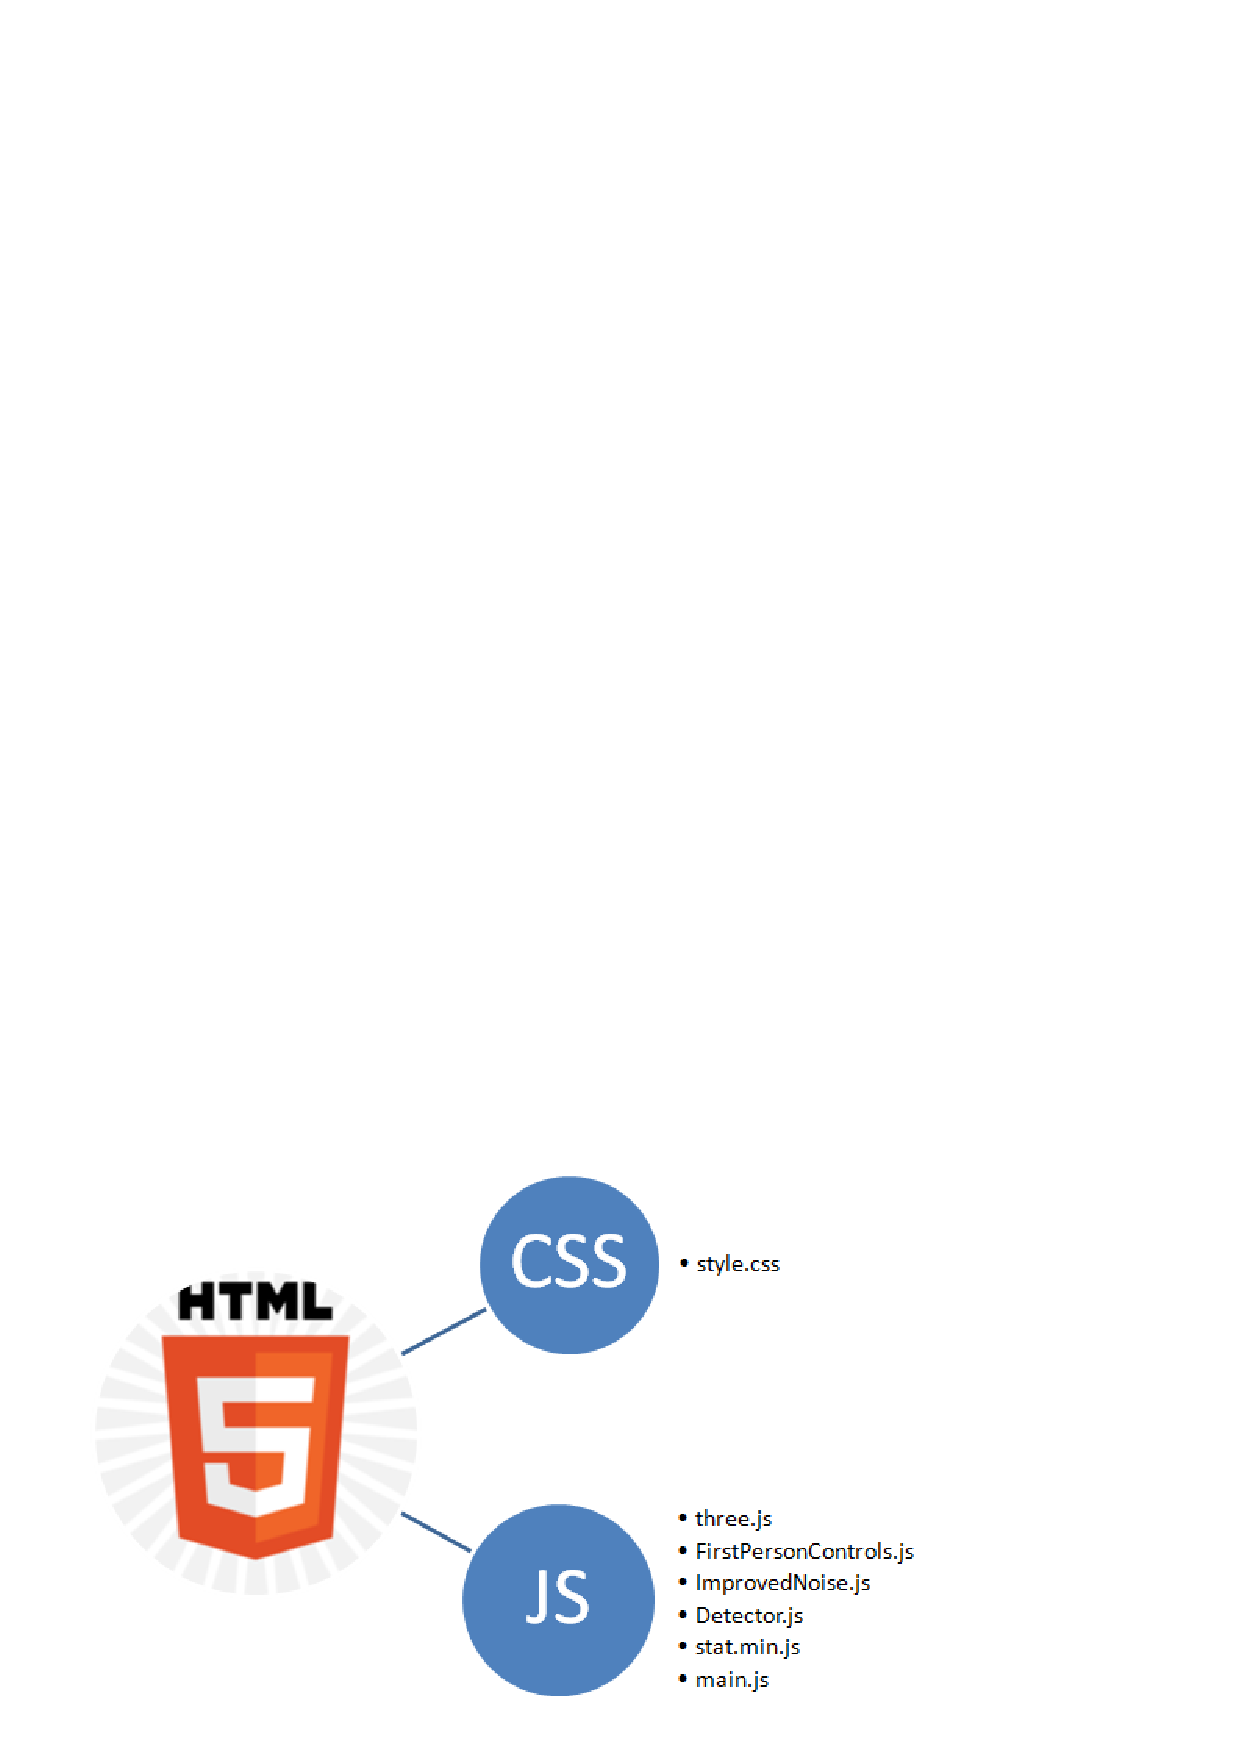
\includegraphics[height=6cm]{images/ProFileOrganisation.png}\\
	\textit{Structure du projet}
\end{center}